En este cap\'itulo se describen las pruebas realizadas al prototipo del sistema de riego para verificar su funcionamiento, as\'i como se comenta los resultados obtenidos de las mismas. 

\section{Pruebas}

\subsection{Control individual de los sensores del sistema de riego con Raspberry}
Inicialmente, para comprobar el funcionamiento de los sensores en Raspberry, cada uno de ellos se prob\'o individualmente en la tarjeta. Para realizar lo anterior, a cada sensor se le asignaron unos pines de uso, de forma que en un futuro pudieran integrarse todos juntos sin problema, y se les dise\~{n} un peque\~{n}o script sin interfaz gr\'afica que se encargara de obtener y mostrar los datos del mismo.\\\\
En la figura \ref{r1}, se puede observar el proceso de desarollo de uno de los scripts, todo est\'o dentro de la misma Raspberry.
\begin{figure}[H]
\begin{center}
	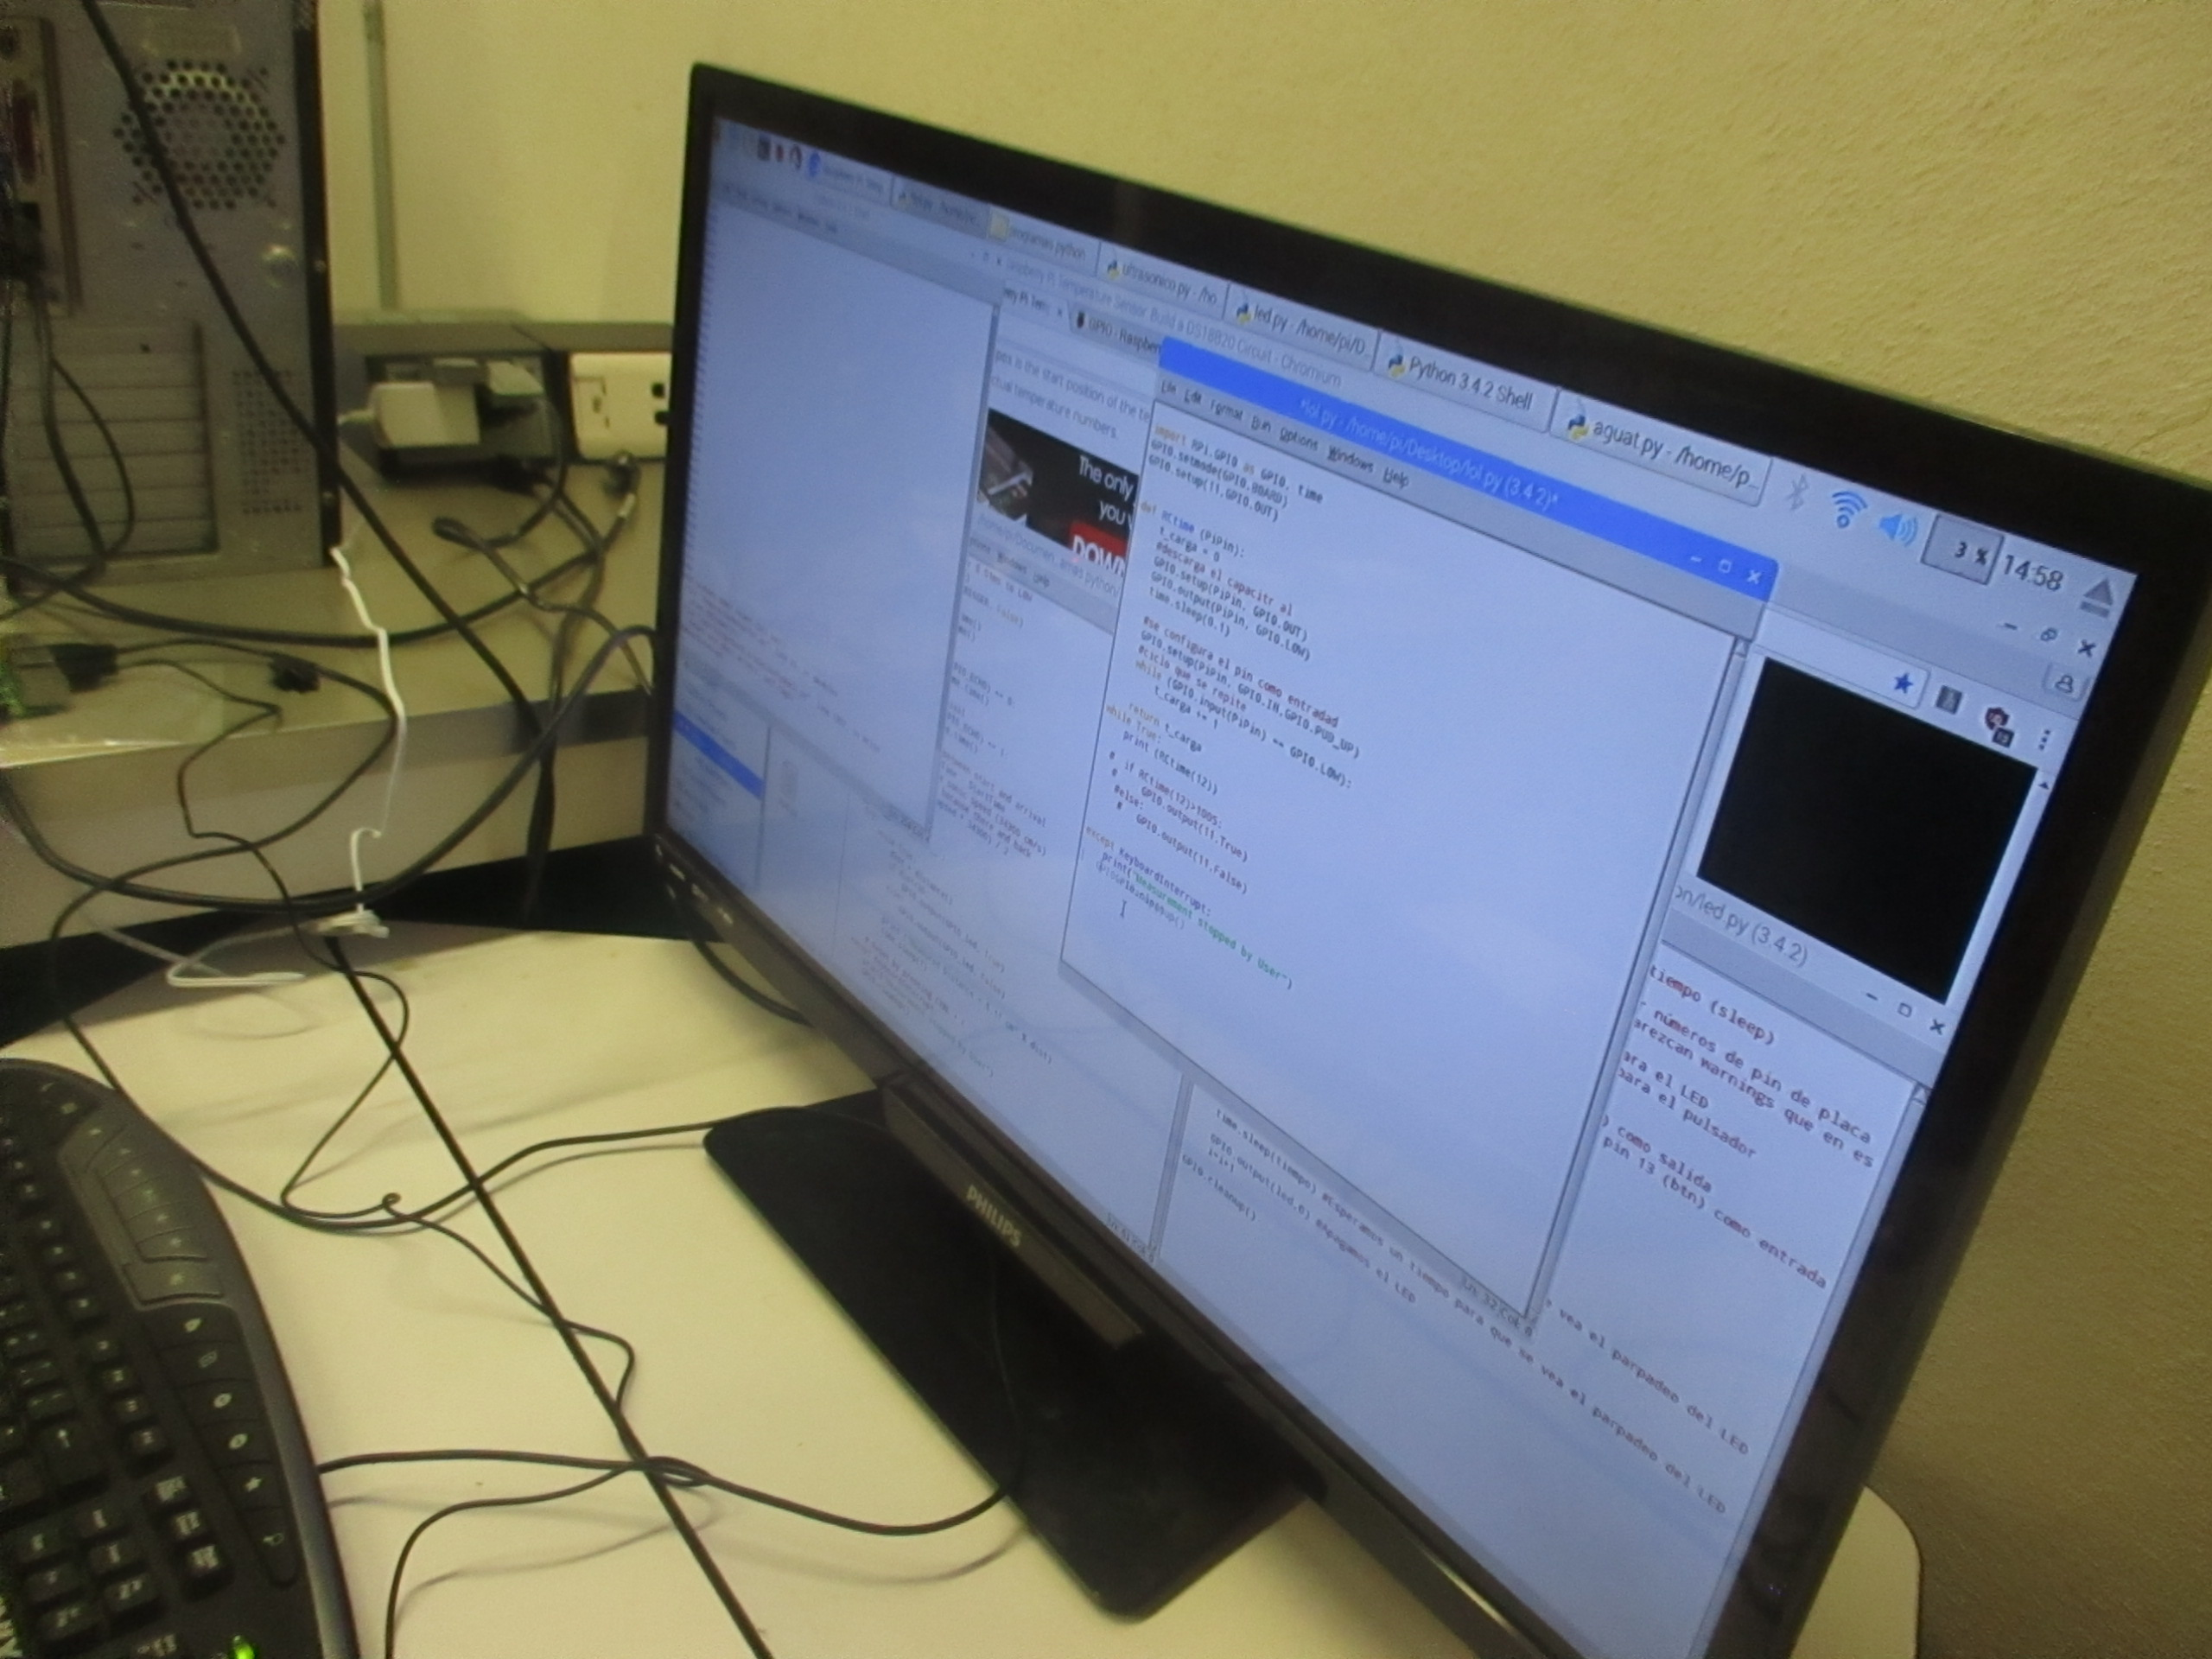
\includegraphics[width=7cm]{r1}
\end{center}
	\caption{Desarrollo del script para el sensor de flujo de agua.}
	\label{r1}
\end{figure} 
El resultado de ejecutar el script anterior, es mostrado en la figura \ref{r4}. El programa corresponde al sensor de flujo de agua y se encarga de mostrar la velocidad del paso de agua de litros por minuto.
\begin{figure}[H]
	\begin{center}
		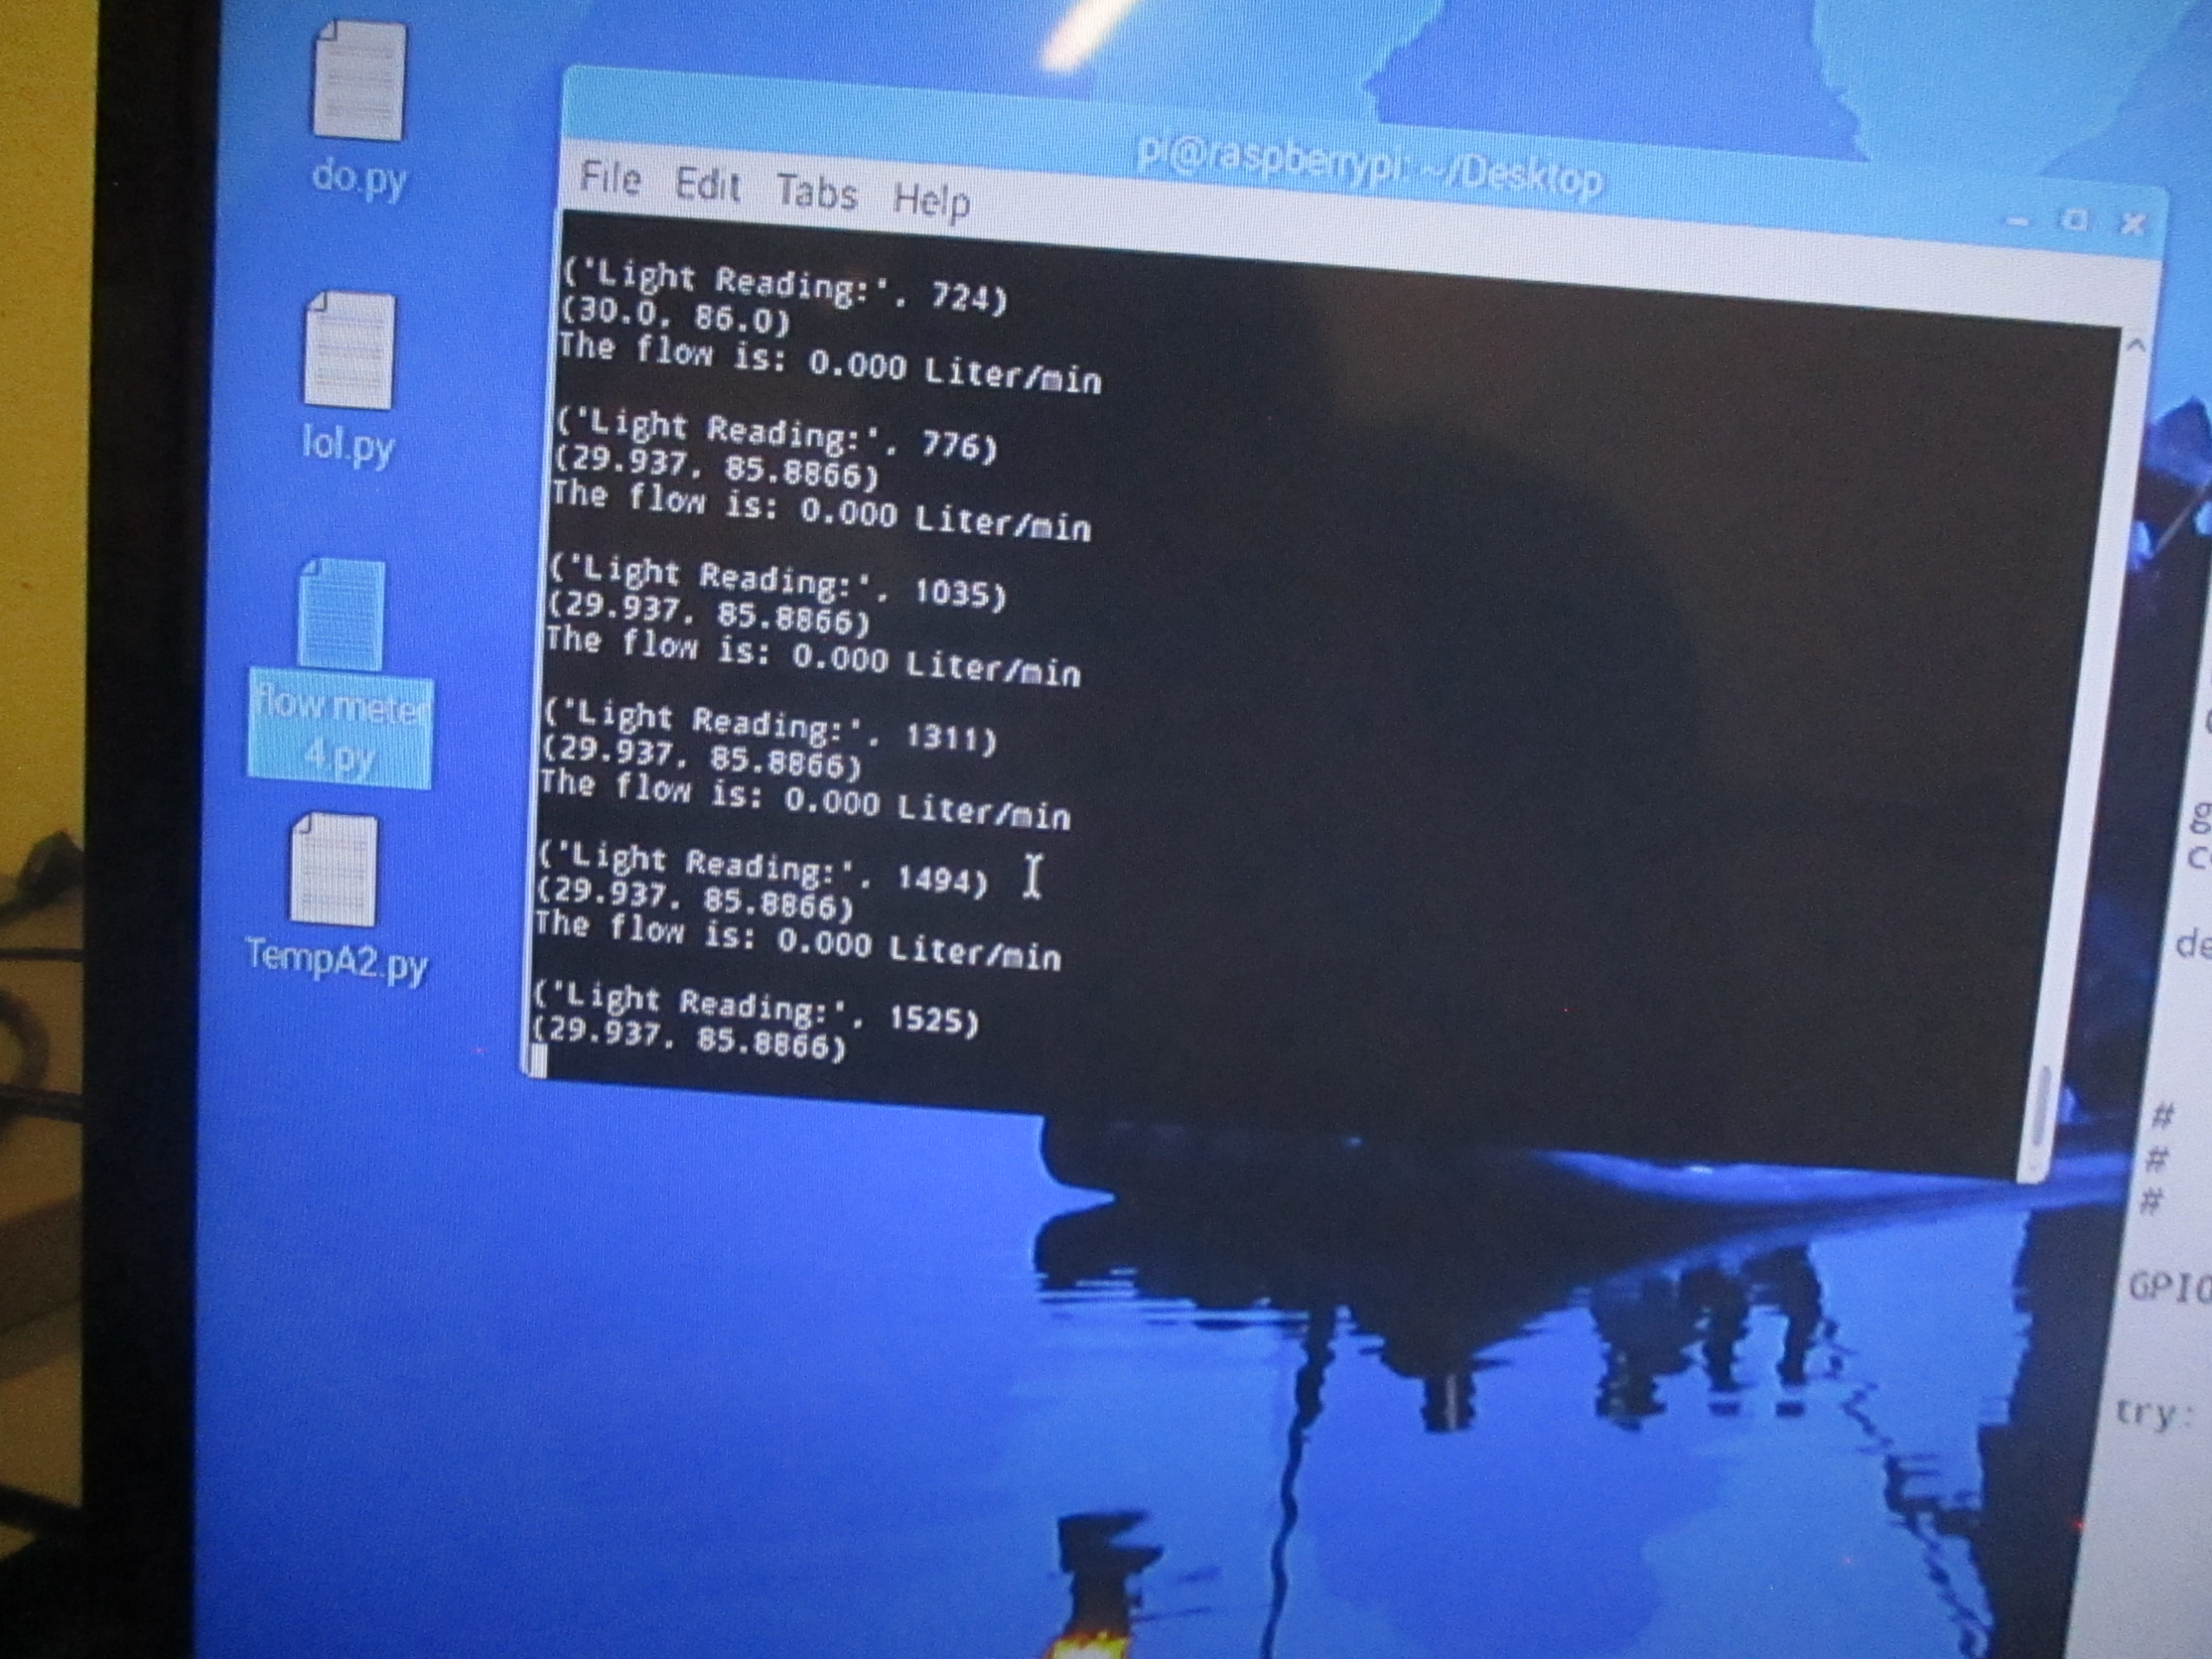
\includegraphics[width=7cm]{r4}
	\end{center}
	\caption{Prueba de funcionamiento del script del sensor de flujo de agua.}
	\label{r4}
\end{figure} 

\subsection{Control grupal de los sensores del sistema de riego con Raspberry}
En la siguiente etapa de desarrollo, todos los sensores fueron integrados a la Raspberry. Con base en lo anterior, se realizaron peque\~{n}as pruebas en las que, de uno en uno, cada sensor se acoplaba en su espacio correspondiente en la tarjeta y su codig\'o de funcionamiento era a\~{n}adido a un script maestro.\\ 
El dise\~{n}o inicial de la Raspberry con todos los sensores integrados puede ser observado en la imagen \ref{todo} (a), mientras que la primera versi\'on del script maestro se puede visualizar en la imagen \ref{todo} (b). 
 
\begin{figure}[H]
	\begin{center}
		\subfigure[Sensores conectados a la Raspberry.]{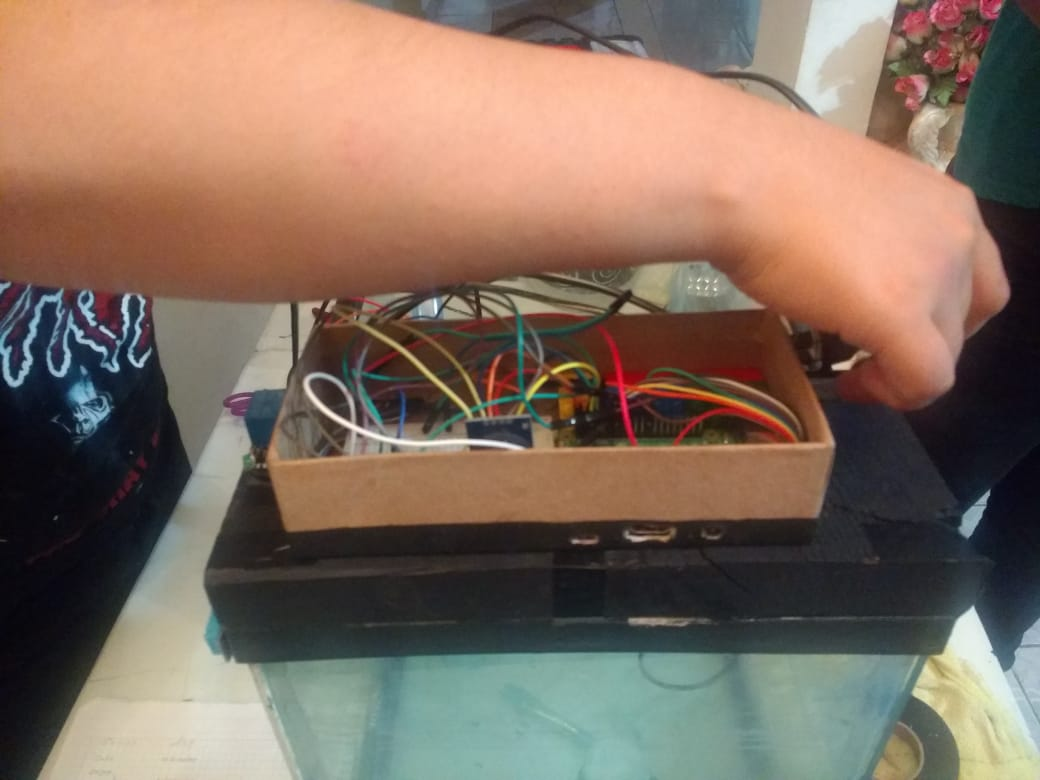
\includegraphics[width=7.5cm]{proto2}}
		\subfigure[Funcionamiento del script maestro.]{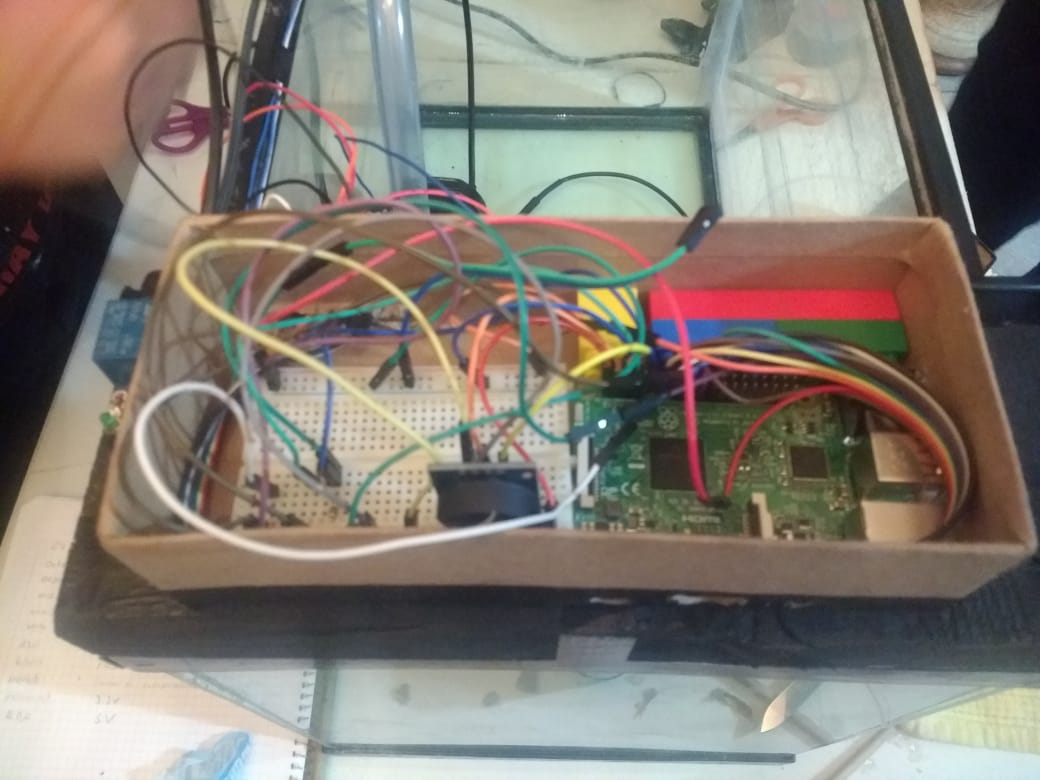
\includegraphics[width=7.5cm]{proto1}}
	\end{center}
	\label{todo}
	\caption{Primera versi\'on del prototipo de sistema de riego}
\end{figure} 


\subsection{Interpretaci\'{o}n de los datos obtenidos de los sensores del sistema de riego con Raspberry}
En las \'ultimas fases de desarrollo, con la Raspberry censando de manera correcta las variables del entorno, se empez\'o a desarrollar un codig\'o para la interpretaci\'on de los datos obtenidos. Por ejemplo: si la humedad en el suelo es muy baja el riego comienza, en caso contrario el riego se detiene; si el nivel de agua disponible es muy bajo, el prototipo no acciona la bomba y manda un mensaje al usuario inform\'andole de lo acontecido. Para probar que lo anterior dicho sucede, se recrearon las condiciones necesarias para que cada uno de estos eventos suceda.

\begin{comment} 
Se puede observar en la imagen \ref{evento1} que, cuando el sensor de humedad del suelo reporta valores altos, el riego se detiene en el momento. 

\begin{figure}[H]
	\begin{center}
		\subfigure[Detecci\'on de un nivel alto de humedad del suelo.]{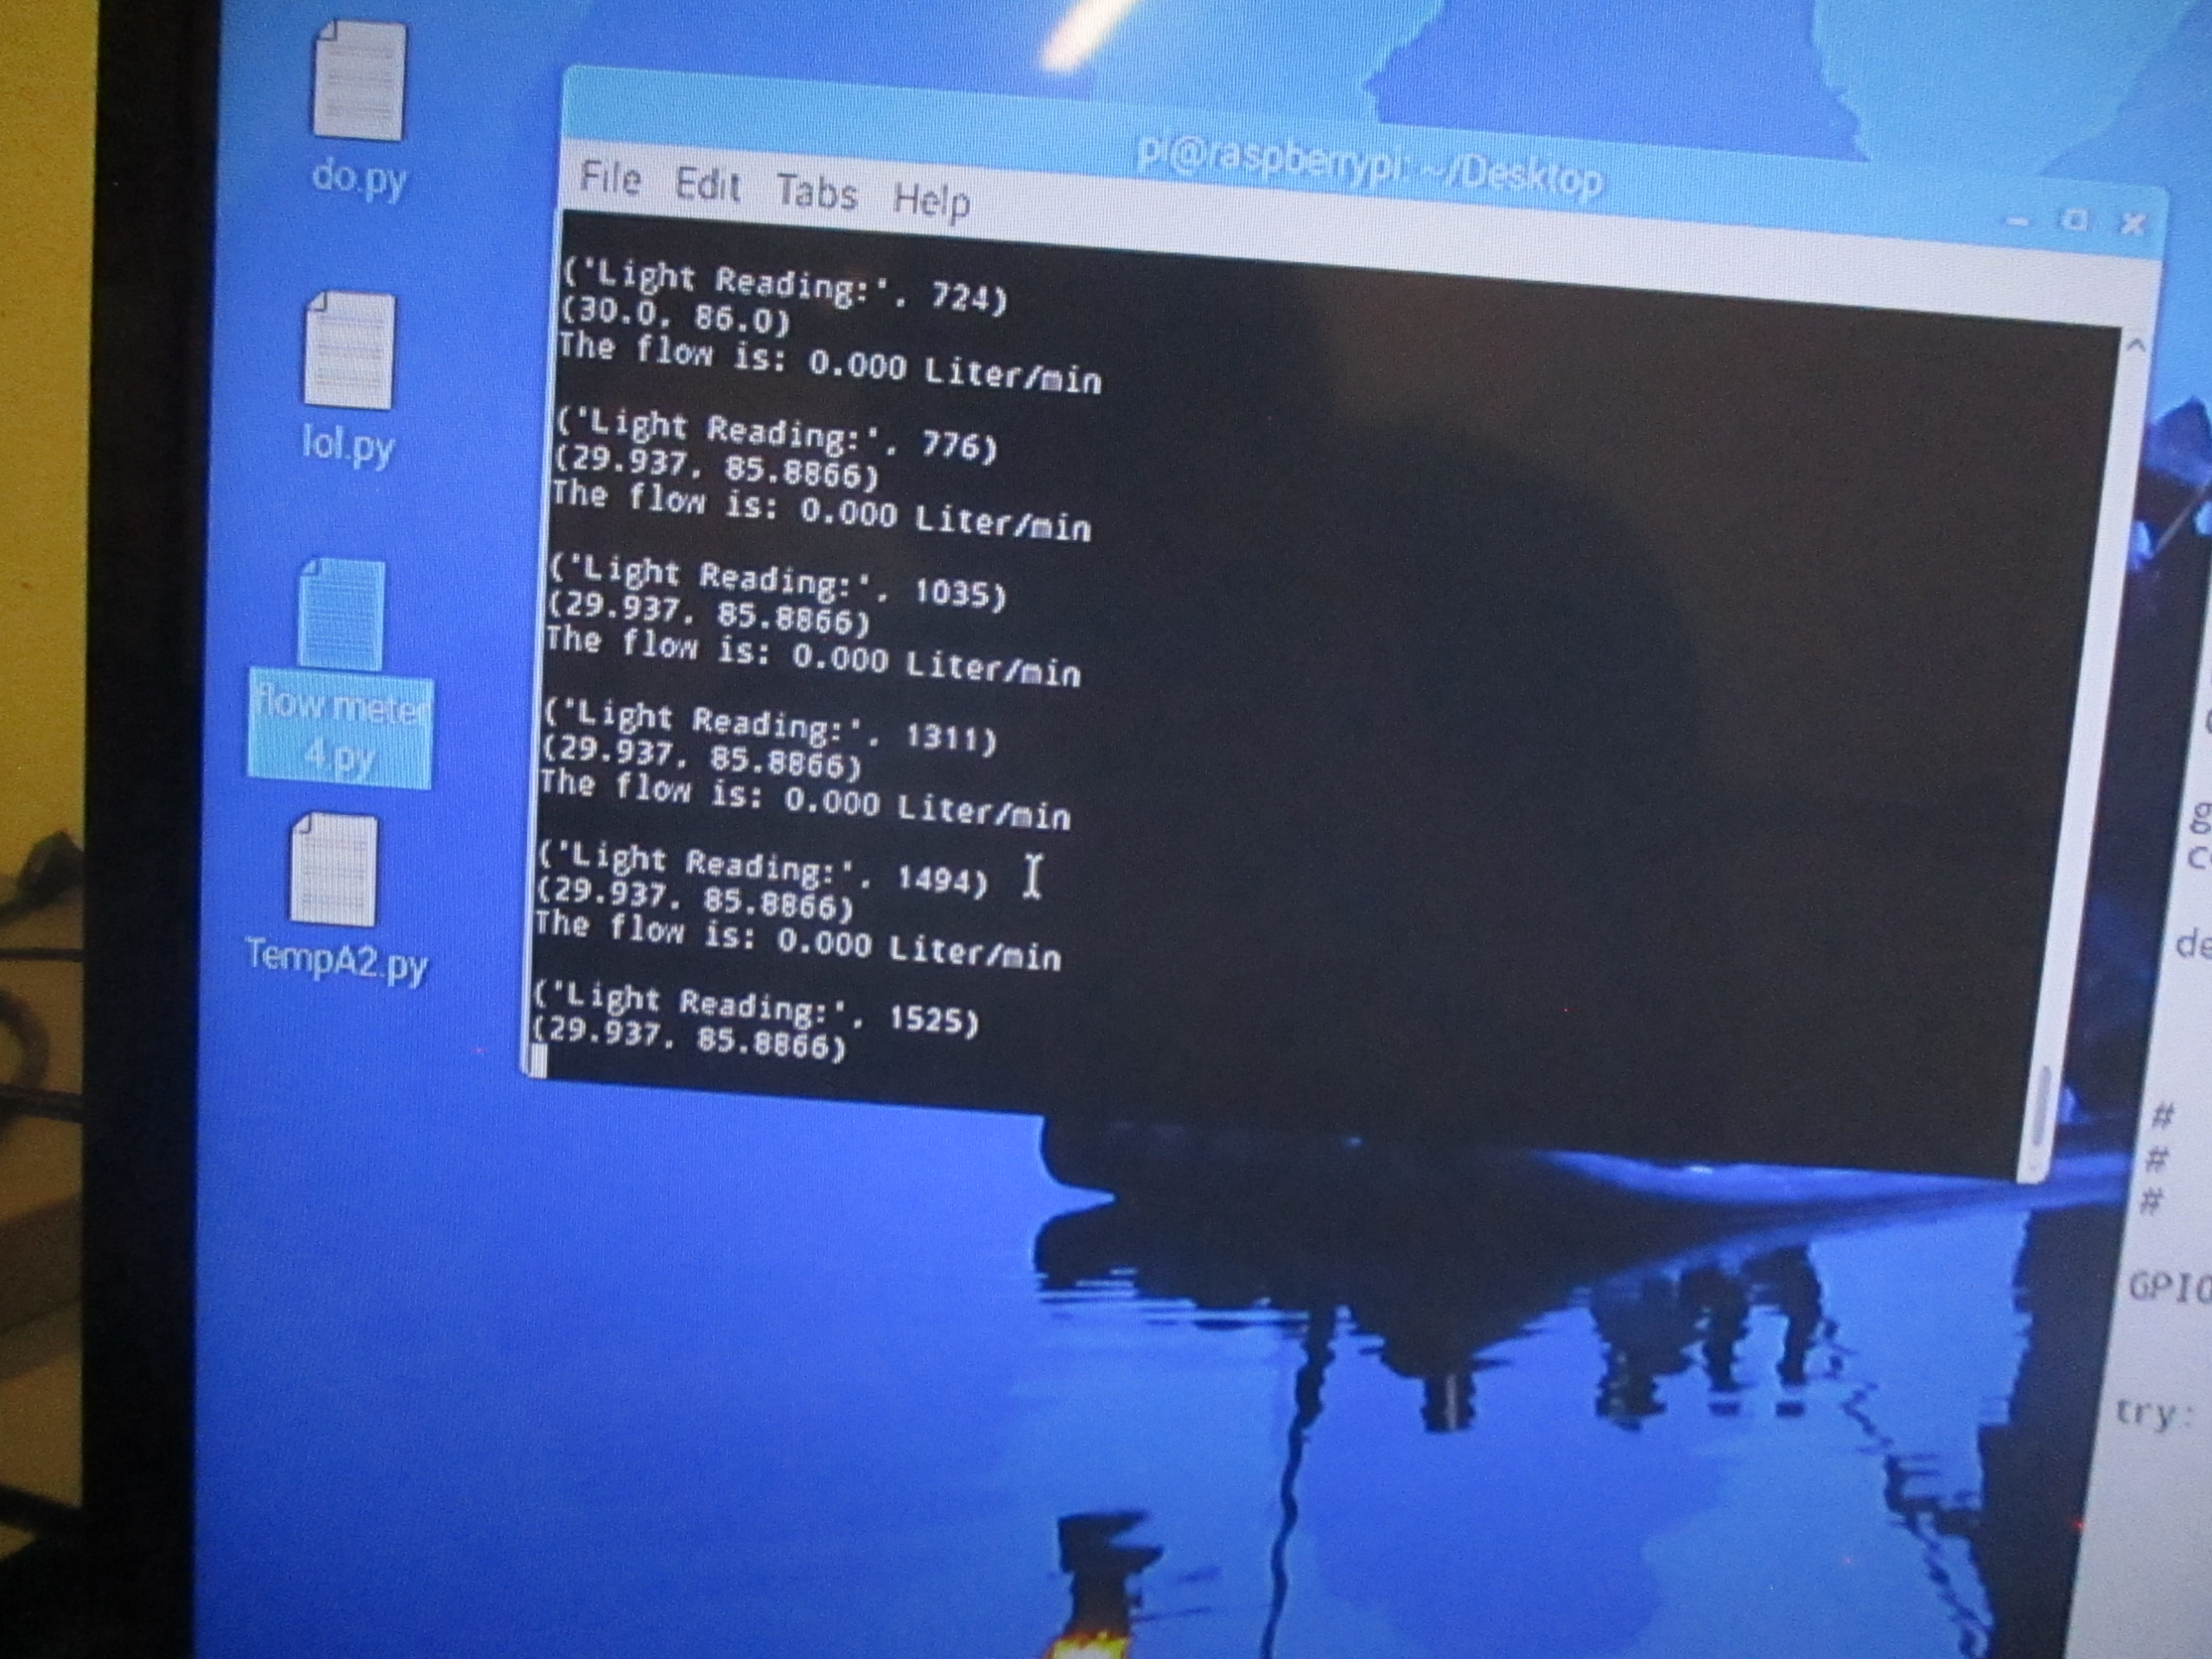
\includegraphics[width=7.5cm]{r4}}
		\subfigure[Riego detenido.]{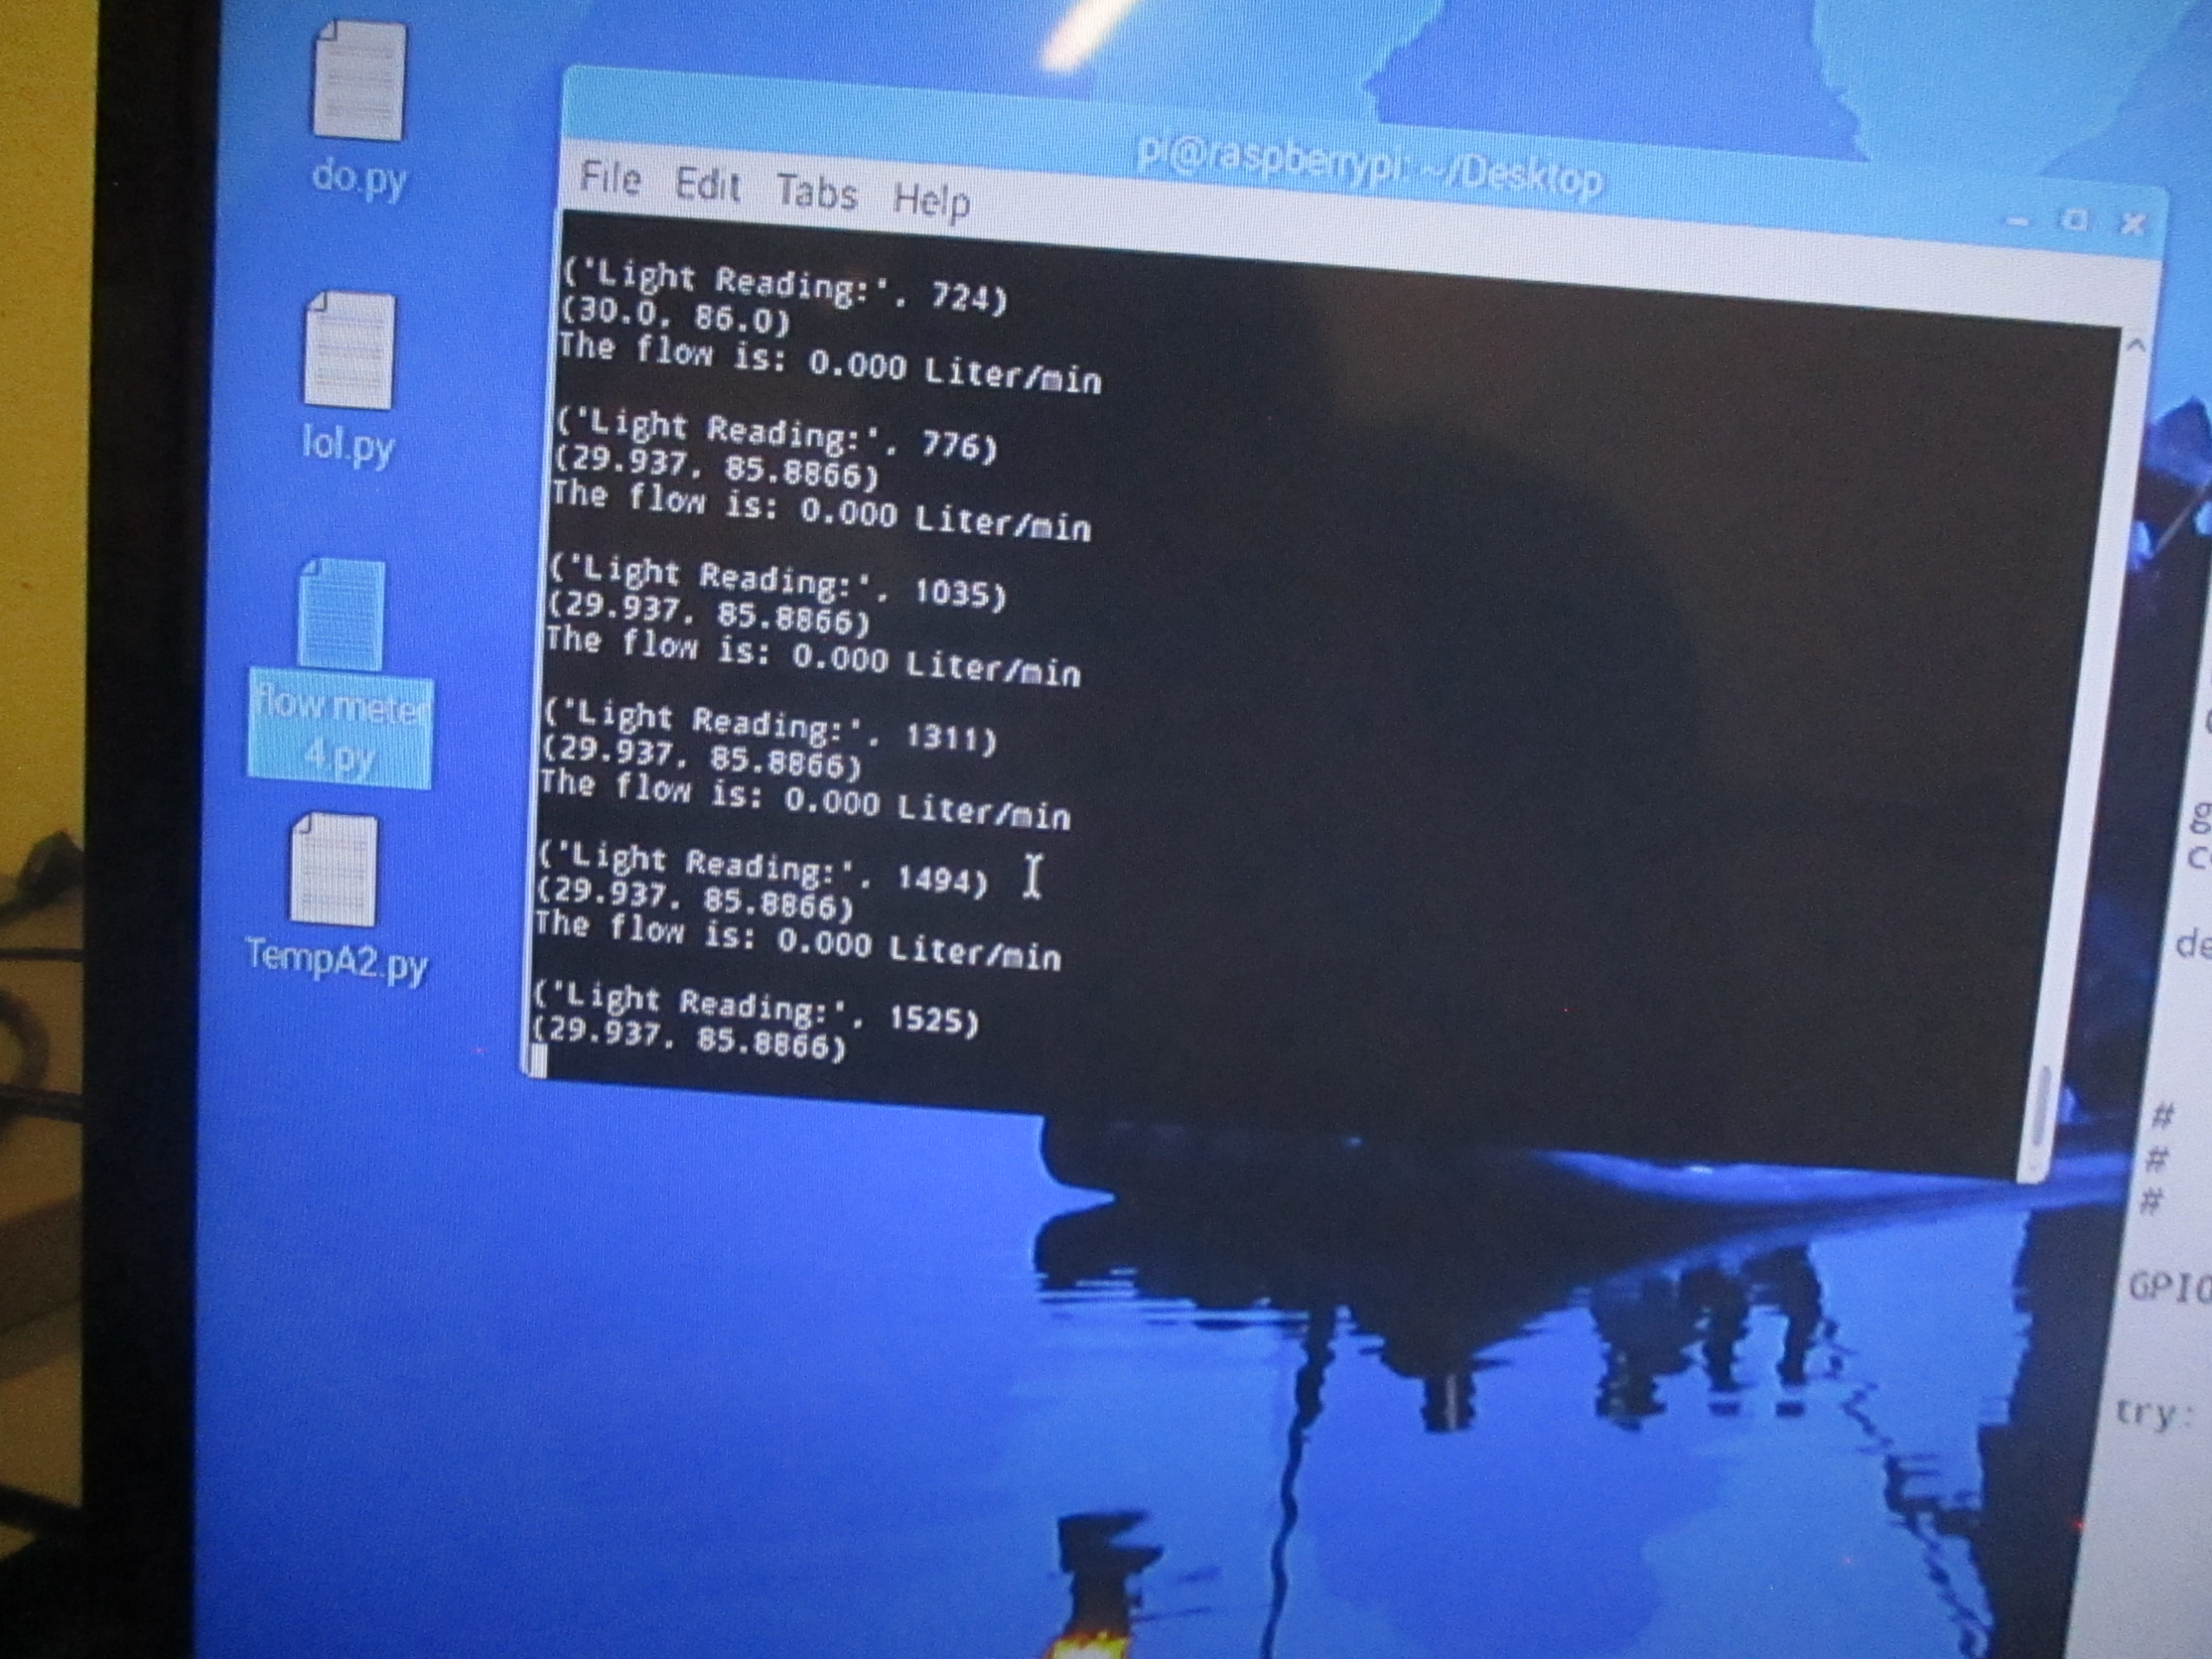
\includegraphics[width=7.5cm]{r4}}
	\end{center}
	\label{evento1}
	\caption{Primera evento considerado.}
\end{figure} 

En caso de que se detecten valores bajos de humedad en el suelo como en la imagen \ref{evento2}, el riego dar\'a inicio de manera autom\'atica. 

\begin{figure}[H]
	\begin{center}
		\subfigure[Detecci\'on de un nivel bajo de humedad del suelo.]{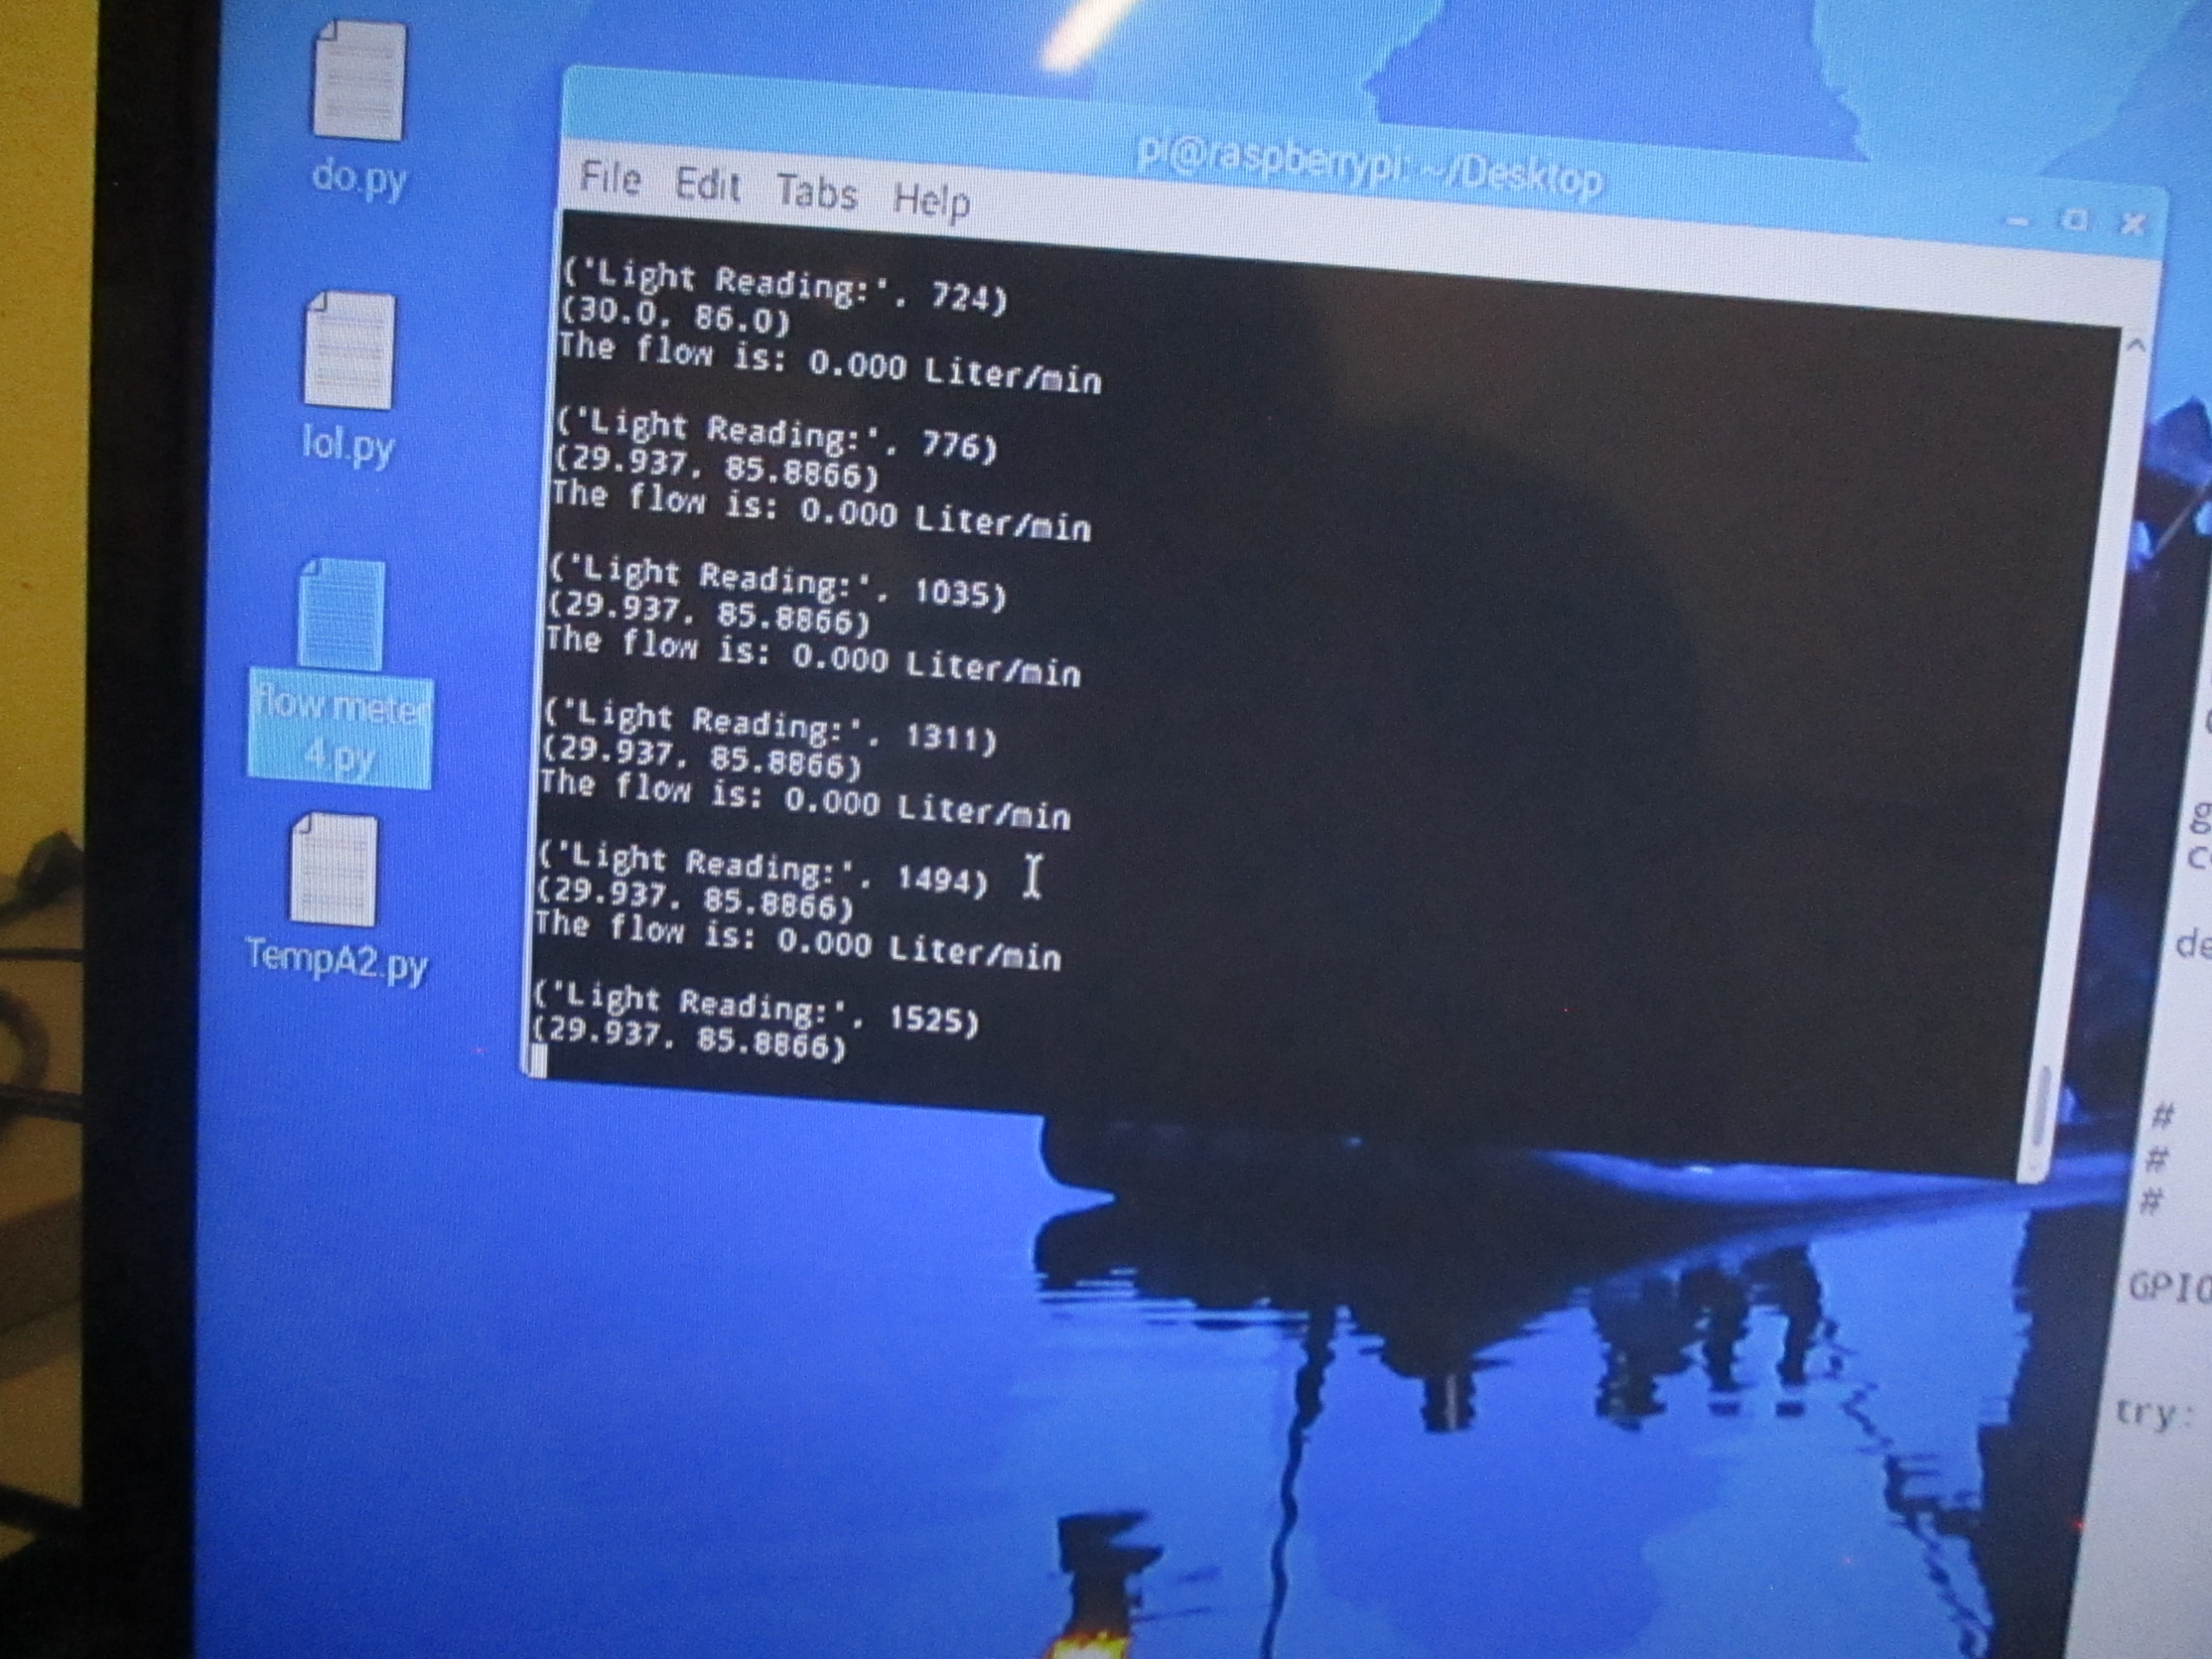
\includegraphics[width=7.5cm]{r4}}
		\subfigure[Riego detenido.]{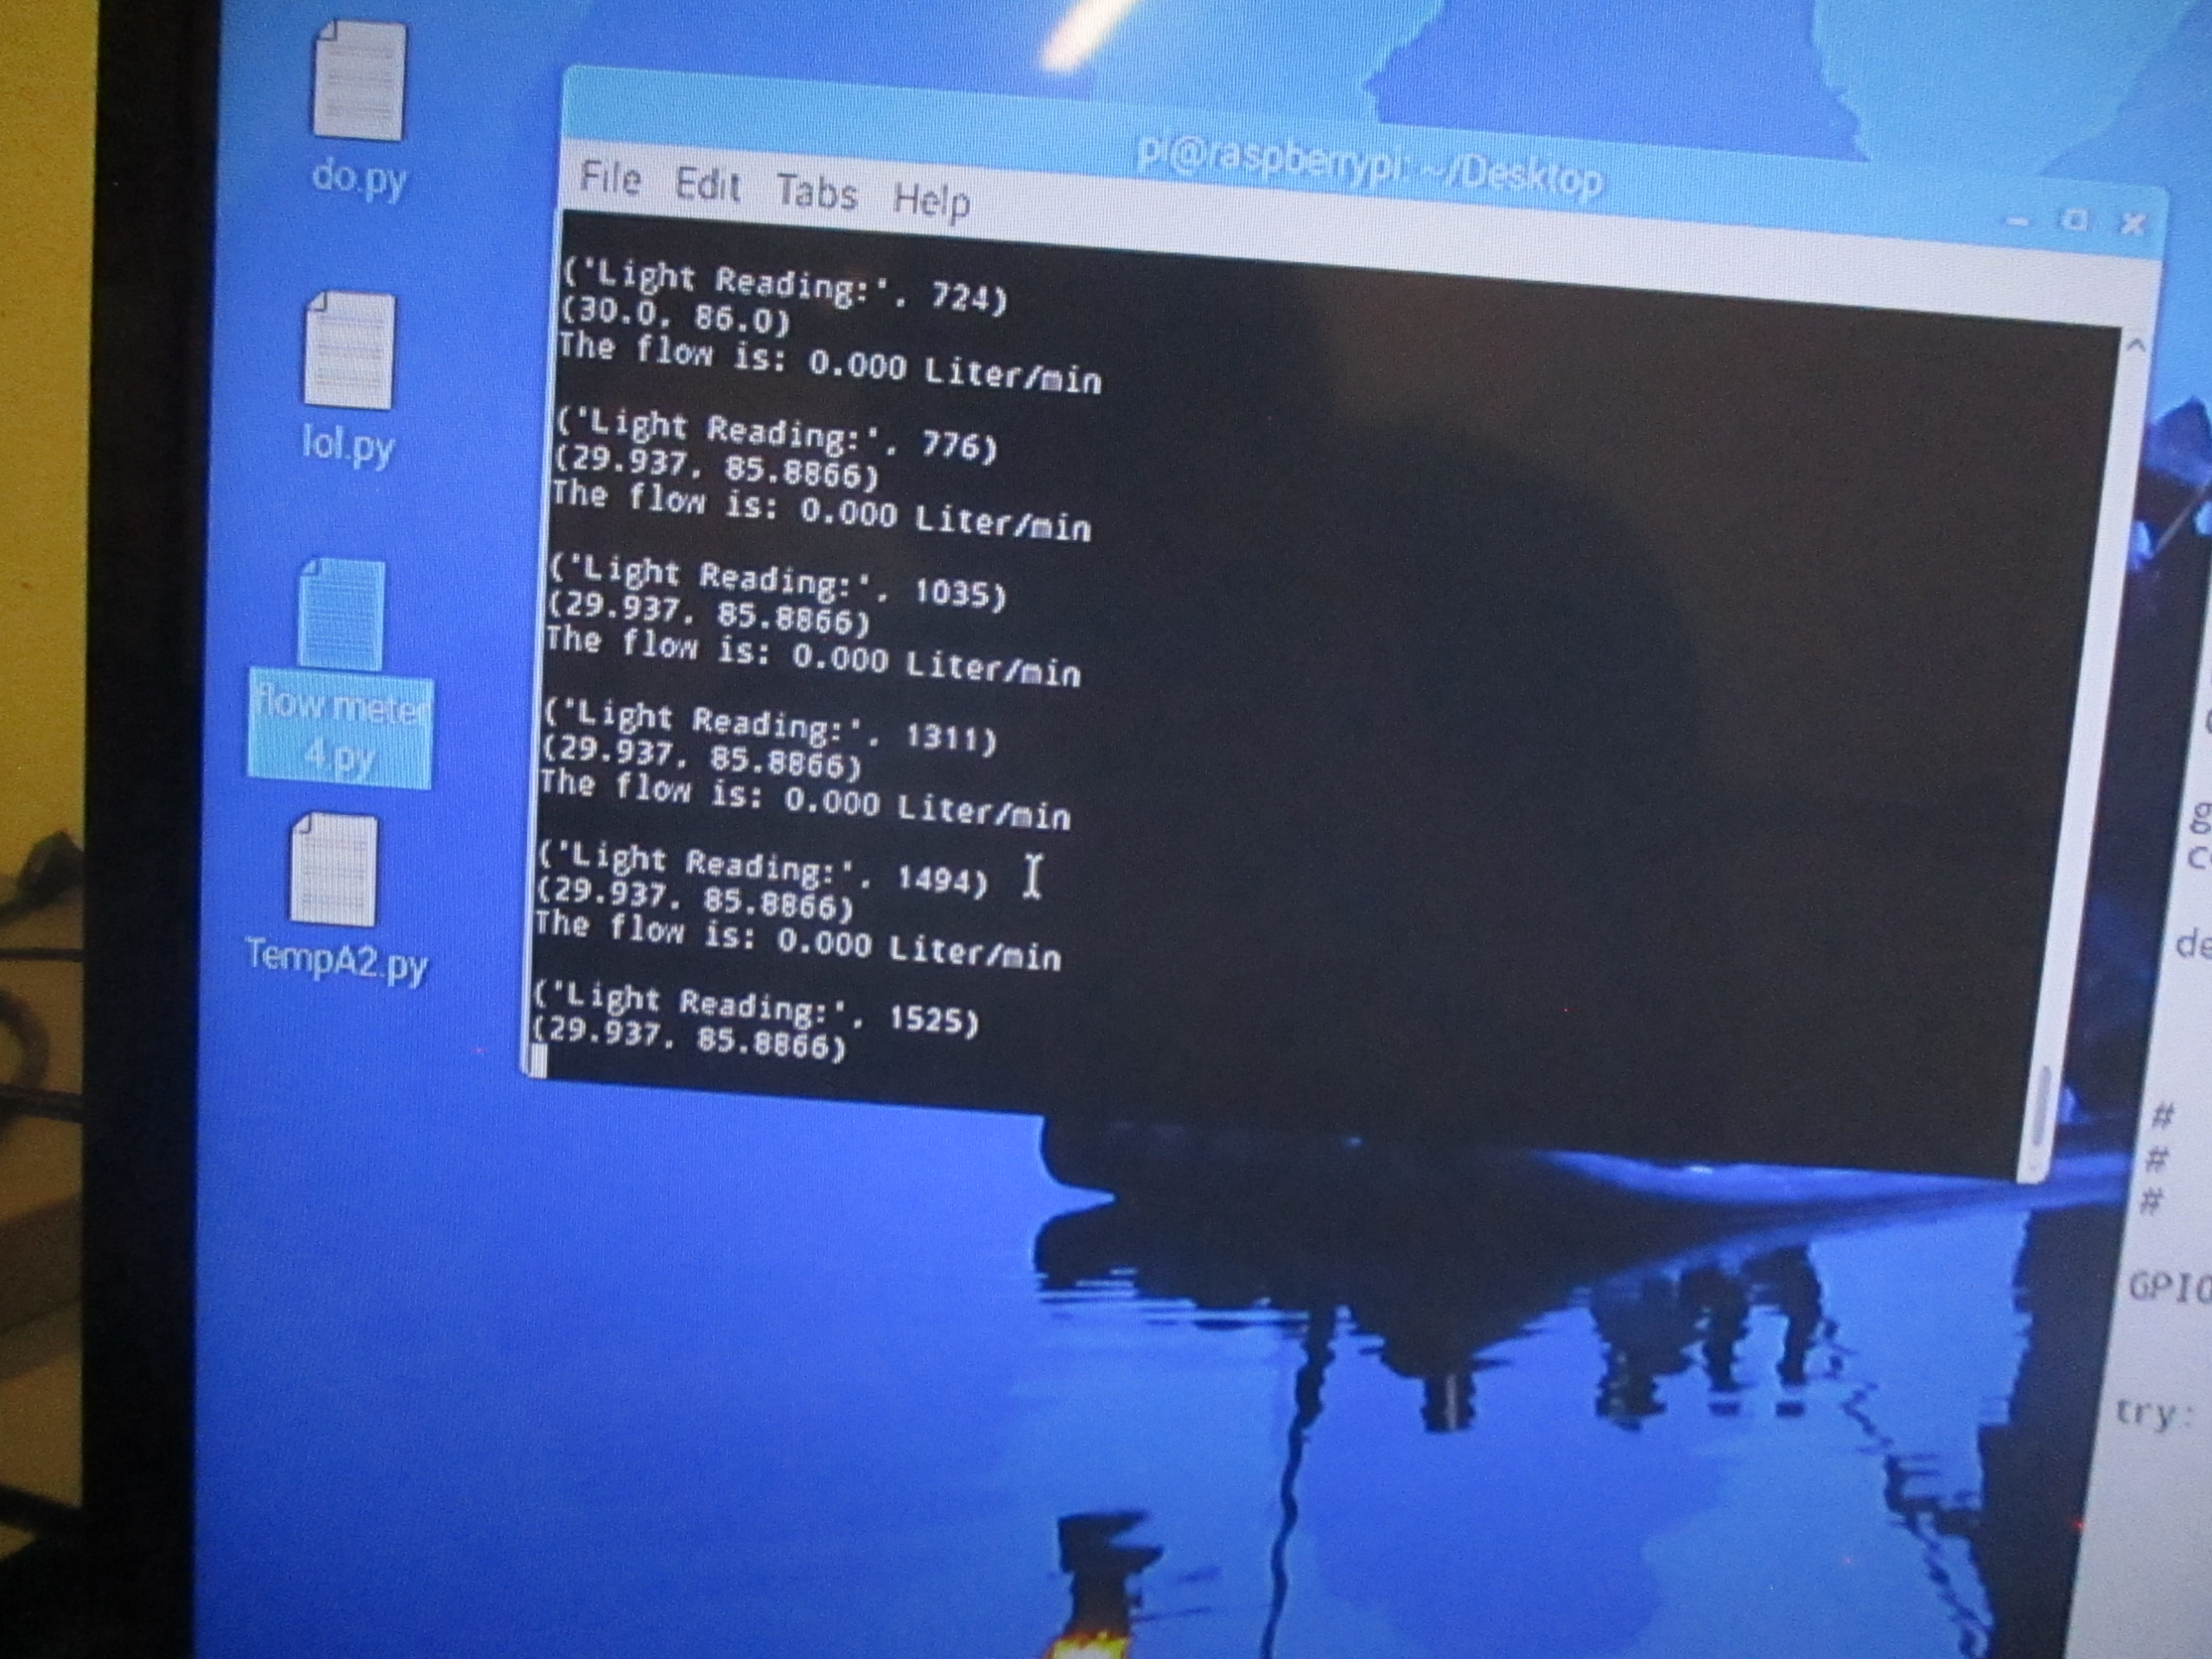
\includegraphics[width=7.5cm]{r4}}
	\end{center}
	\label{evento2}
	\caption{Segundo evento considerado.}
\end{figure} 

Otra forma de detener el flujo de agua, es detectando un nivel de agua bajo parecido al de la imagen \ref{event3}.  

\begin{figure}[H]
	\begin{center}
		\subfigure[Detecci\'on de un bajo nivel de agua.]{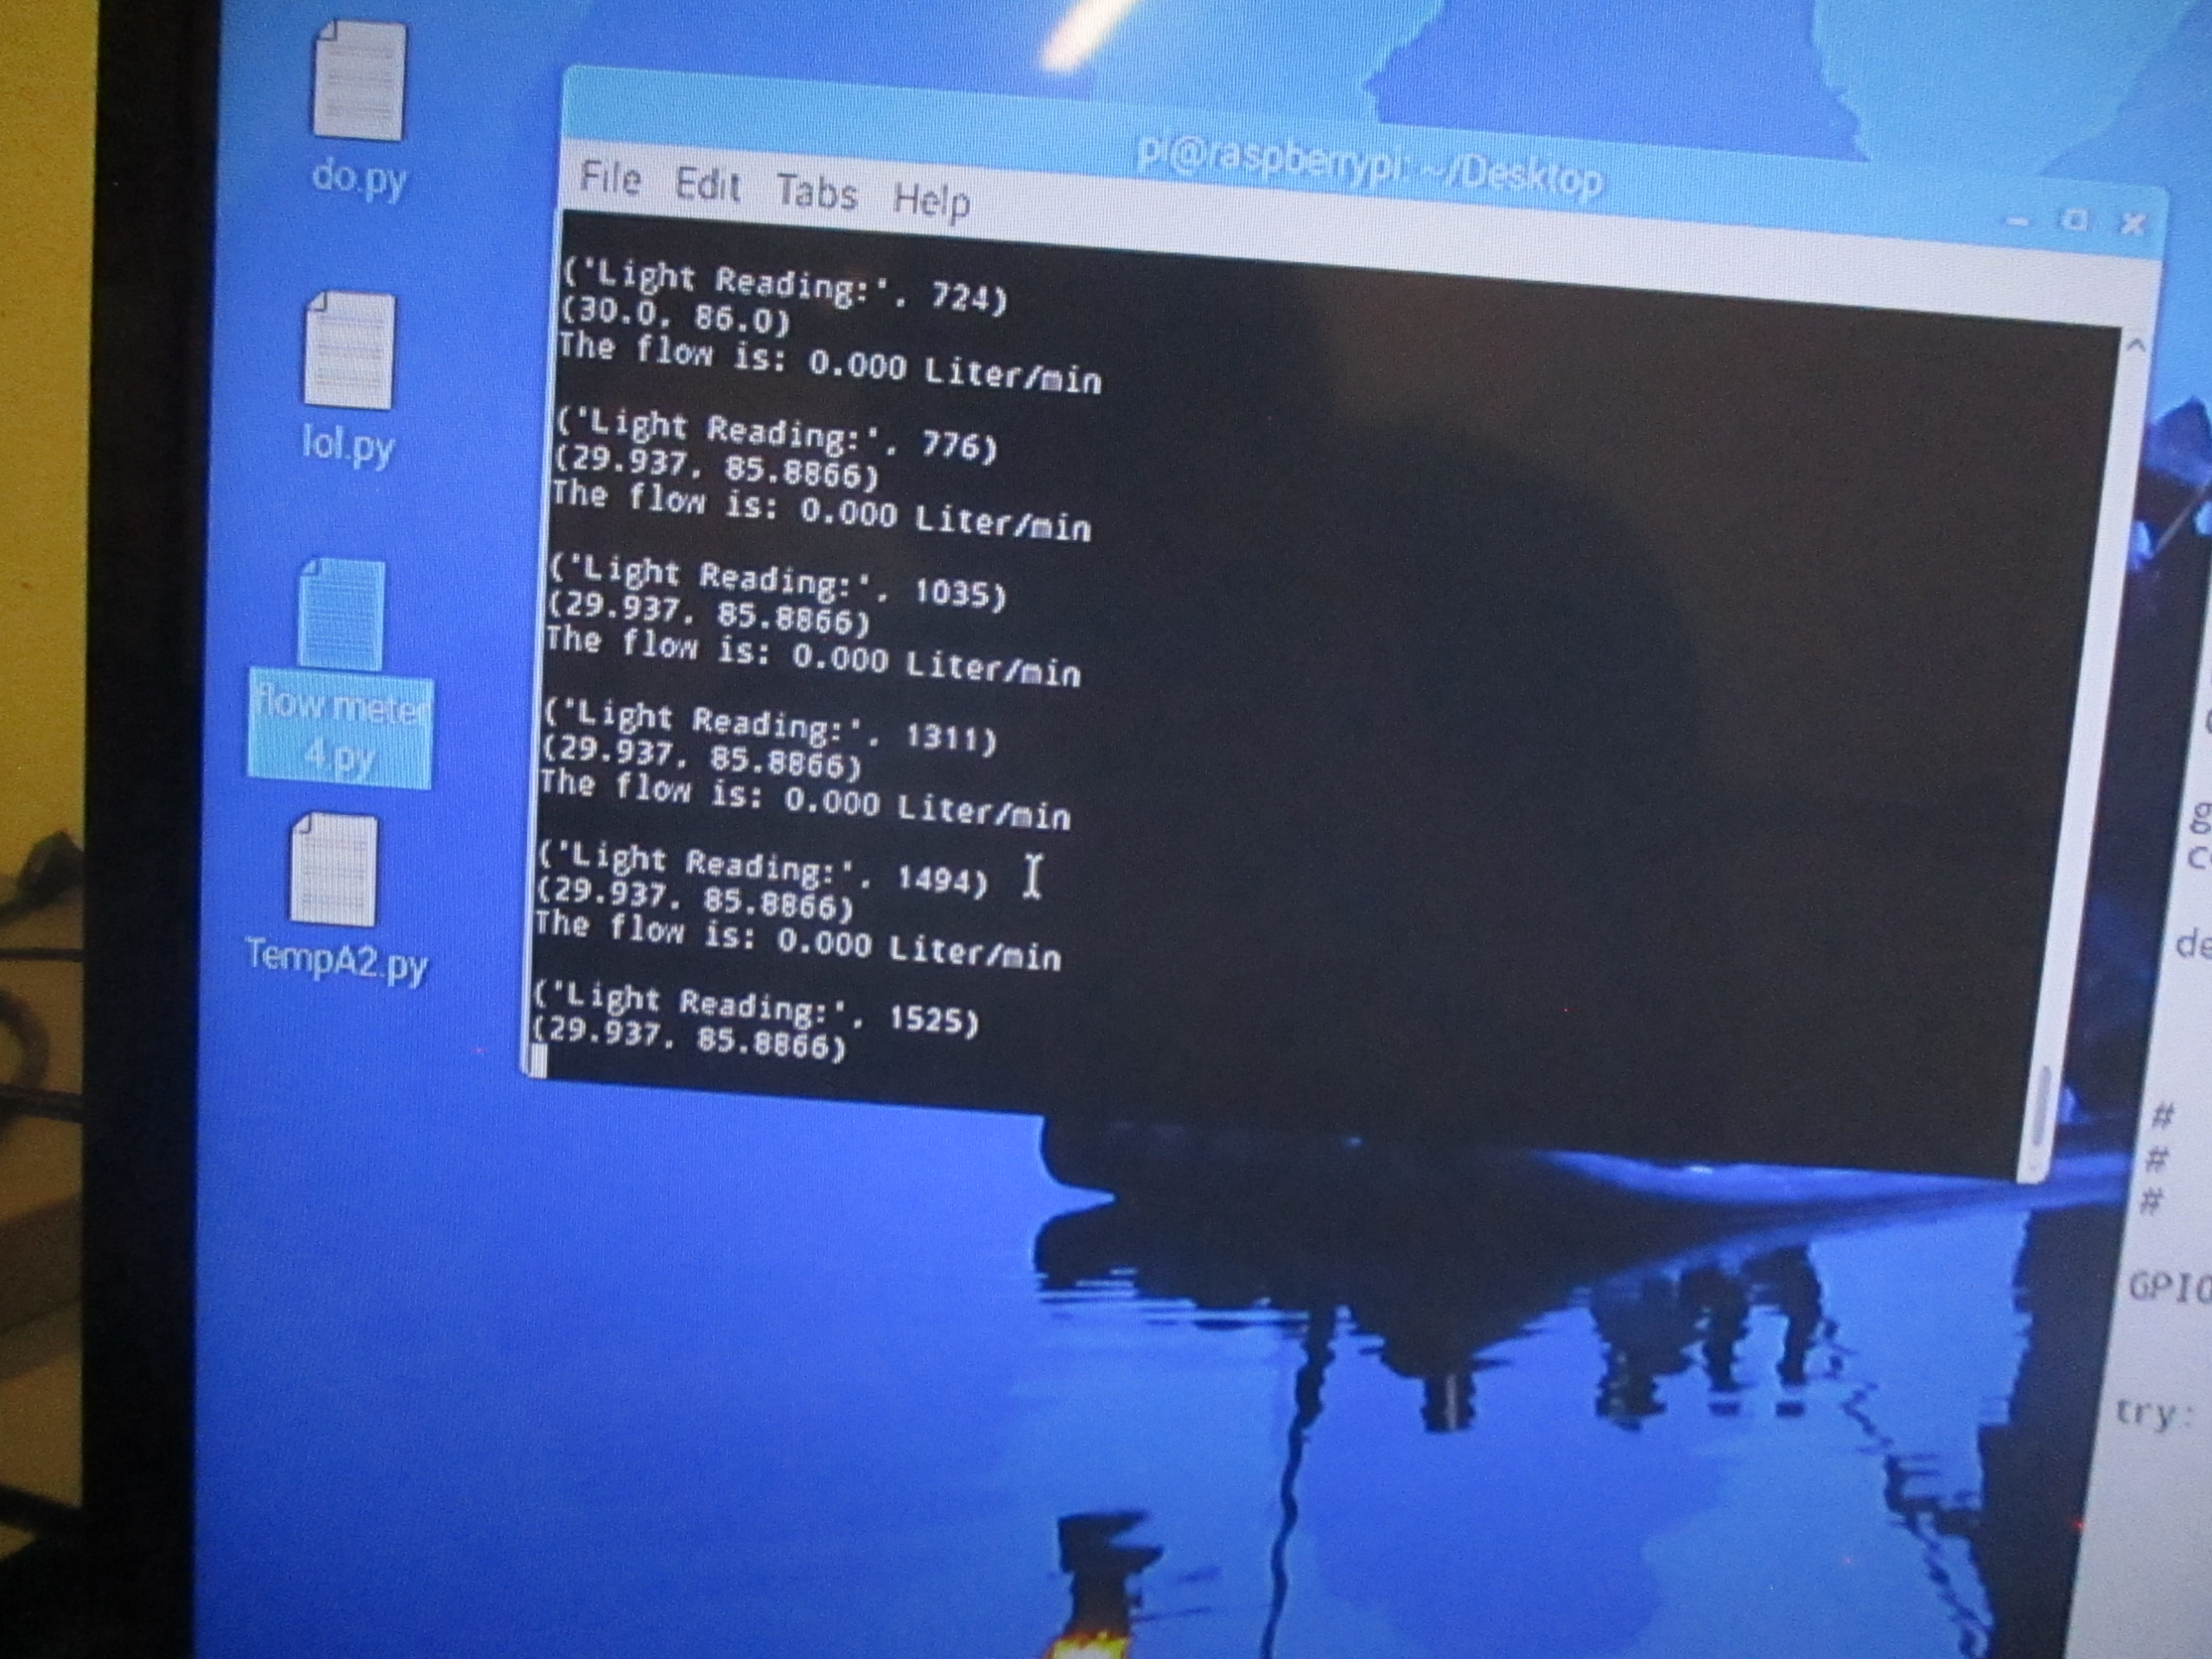
\includegraphics[width=7.5cm]{r4}}
		\subfigure[Riego detenido.]{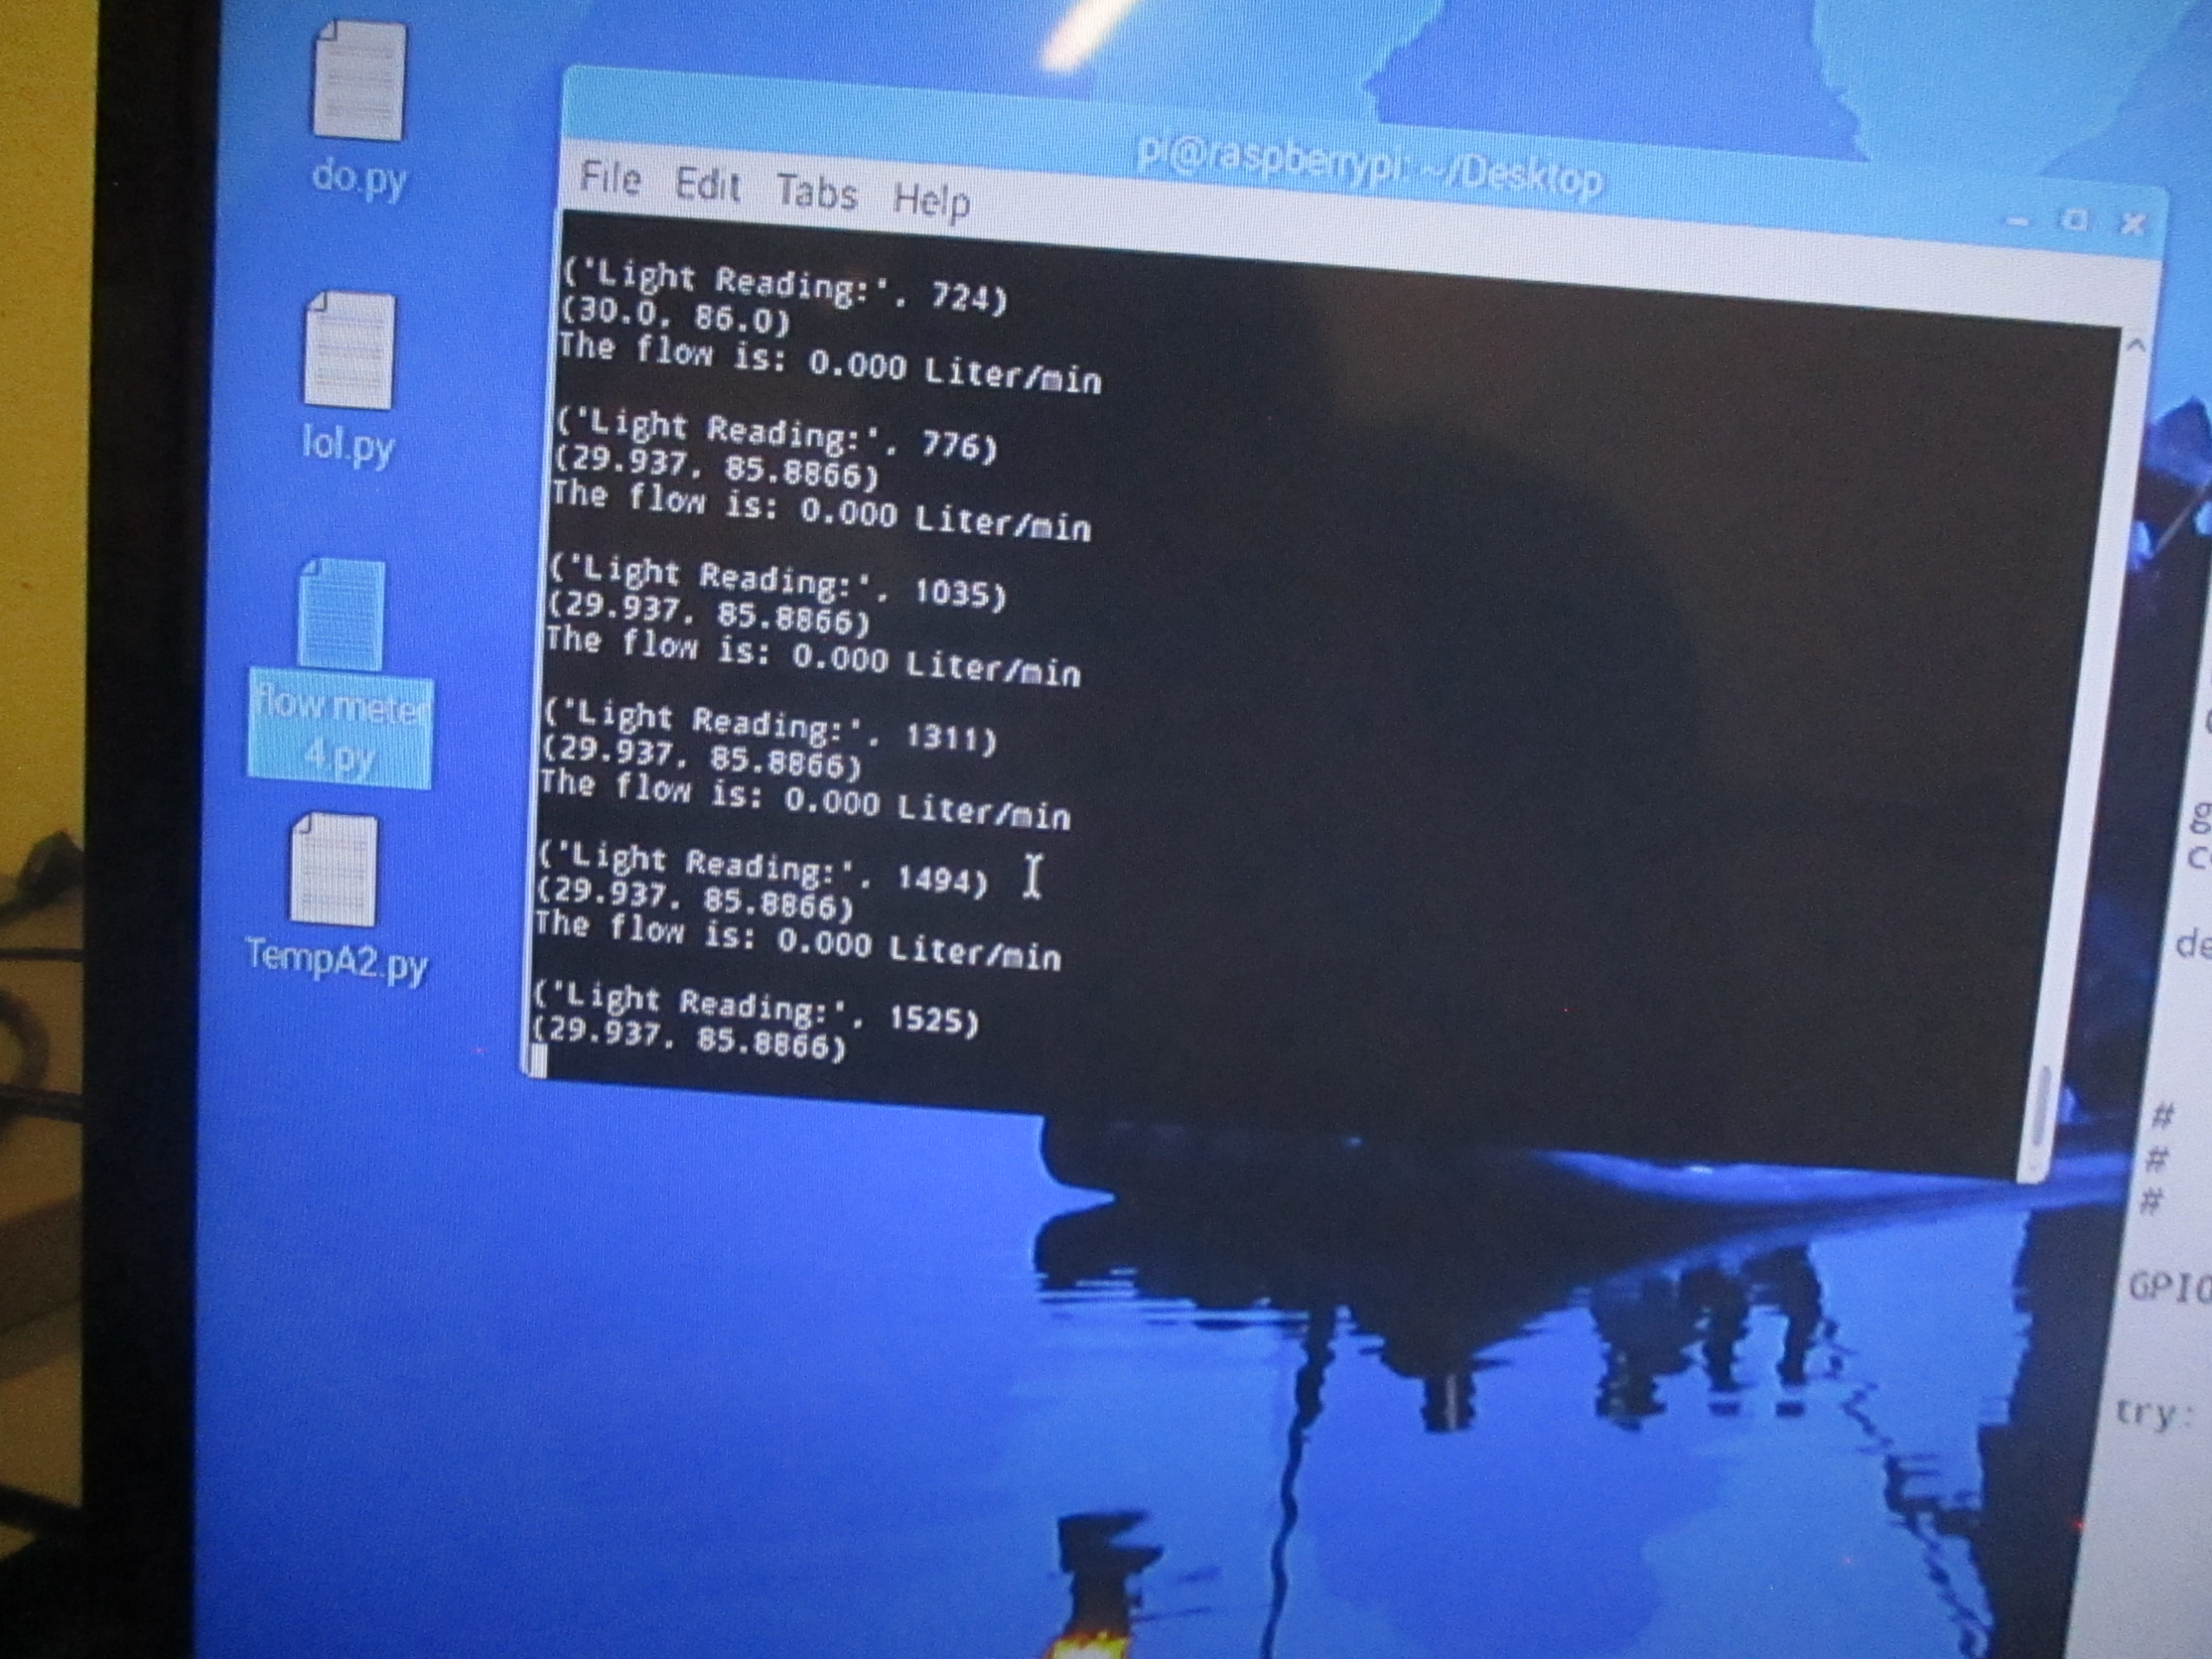
\includegraphics[width=7.5cm]{r4}}
	\end{center}
	\label{event3}
	\caption{Tercer evento considerado.}
\end{figure} 

\end{comment}

\section{Resultados}
El prototipo del sistema de riego supero satisfactoriamente las pruebas a las que fue sometido, demostrando as\'i, su eficiencia en cuanto a recopilaci\'on e interpretaci\'on de datos se refiere.\\ 
Como resultado de las pruebas, el prototipo sufrio constantes modificaciones de dise\~{n}o tanto en la parte hardware como en la parte de software. En lo que respecta al hardware, todo el sistema critico fue aislado en una caja, con correspondientes adaptaciones a la misma, y montado sobre un tanque de agua con el resto de los sensores ambientales a su alrededor, tal y como se ve en la imagen 5.4.%\ref{hardwareda}. 

\begin{figure}[H]
	\begin{center}
		\subfigure[Exterior del prototipo.]{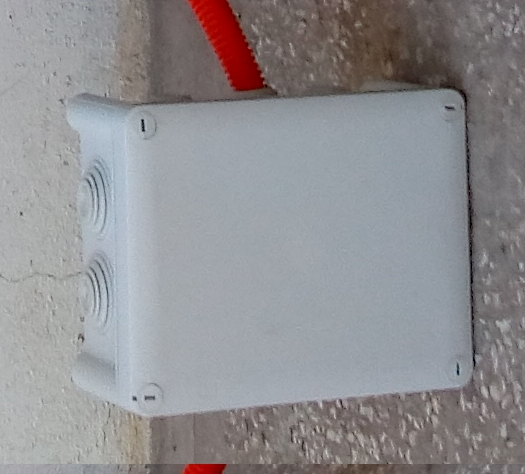
\includegraphics[width=7.5cm]{hardwarec}}
		\subfigure[Interior del prototipo.]{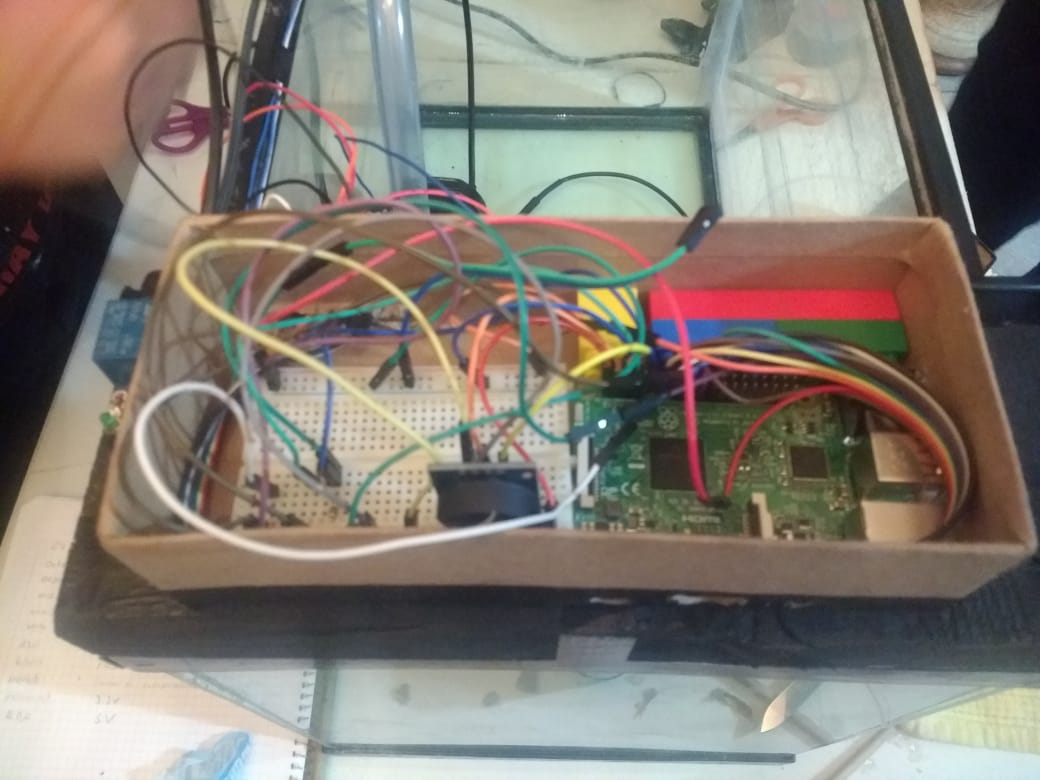
\includegraphics[width=7.5cm]{hardwarea}}
	\end{center}
	\label{hardwareda}
	\caption{Vista del prototipo.}
\end{figure} 

En el caso del software, se desarroll\'o una interfaz gr\'afica simple, de manera que el usuario pueda interactuar con el prototipo de una manera m\'as amigable. La interfaz se puede ver en la imagen \ref{software}.

\begin{figure}[H]
	\begin{center}
		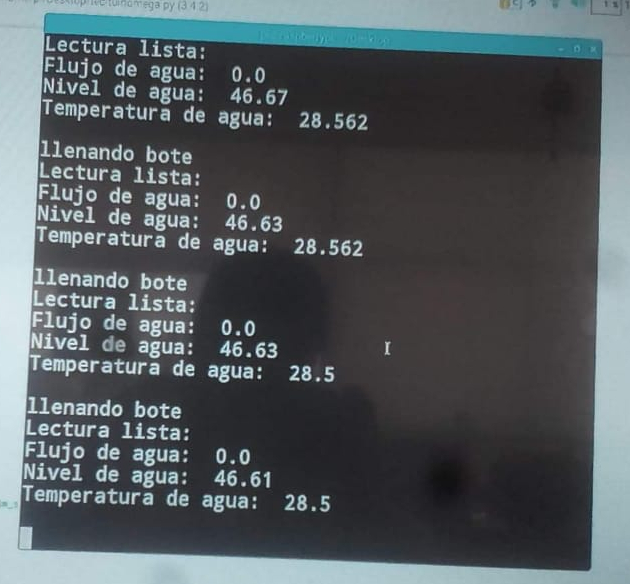
\includegraphics[width=7cm]{software}
	\end{center}
	\caption{Interfaz de usuario del prototipo.}
	\label{software}
\end{figure} 
